\documentclass[main.tex]{subfiles}
\begin{document}


\section{Aufbau des Intrusion Detection Systems}

Das Intrusion Detection System kann grundlegend in zwei Subsysteme unterteilt werden: Einerseits in die Datenaufbereitung, die Data-Preparation, andererseits in die eigentliche Anomalieerkennung, das Intrusion Detection System.
In der Data-Preparation ist es dem Nutzer möglich,aus einer beliebigen Anzahl ausgewählter Szenarien, die zunächst im csv-Format hinterlegt sind, zwei Arff-Dateien zu generieren. Es werden zwei Arff-Dateien generiert, da eine der beiden Dateien zum Trainieren des IDS und die andere Datei zum Testen des IDS vorgesehen sind. Die prozentuale Aufteilung der Daten in Training und Test kann individuell angepasst werden. Die nachfolgende Abbildung gibt einen detaillierten Überblick über den Aufbau der Data-Preparation.\\

%
\begin{figure}[ht]
 \centering
 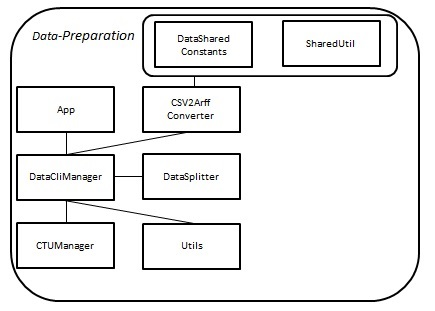
\includegraphics[width=0.65\textwidth]{images/Schema_Data_Preparation.jpg}
 \caption{Schema Data-Preparation}
 \label{schema_data_preparation}
\end{figure}


Im Intrusion Detection System kann der Nutzer zwischen mehreren Classifiern auswählen. Hat der Nutzer einen Classifier ausgewählt und die Parameter gesetzt, trainiert das IDS auf dem in der Data-Preparation vorbereiteten Trainings-Datensatz und testet anschließend auf dem Test-Datensatz. Es ist auch möglich nur ein Training oder nur einen Test durchzuführen. Nachdem das IDS getestet hat, evaluiert es die Testergebnisse. Die Resultate der Evaluierung, die Berechnung der Metriken True Positive, True Negative, False Positive und False Negative werden sowohl in Text- als auch in grafischer Form hinterlegt, um den Nutzer einen Überblick zu verschaffen. 
Die nachfolgende Abbildung gibt einen detaillierten Überblick über den Aufbaudes Intrusion Detection Systems. \\

\begin{figure}[ht]
 \centering
 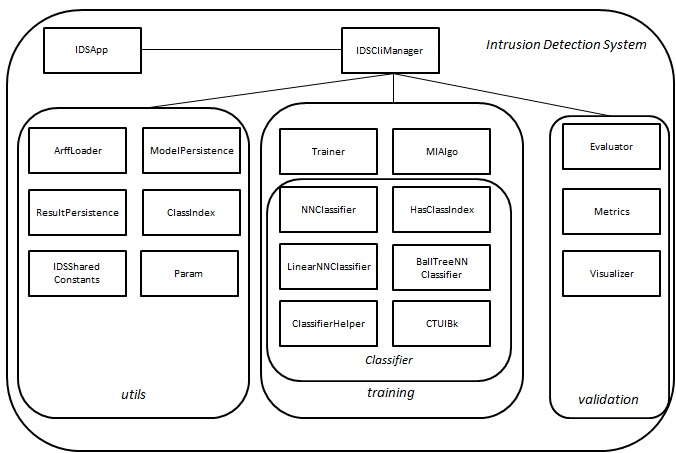
\includegraphics[width=1\textwidth]{images/Schema_IDS.jpg}
 \caption{Schema IDS}
 \label{schema_ids}
\end{figure}


\section{Machine Learning}
\subsection{Classifier}
Für das IDS wurden die Classifier implementiert.


\end{document}

% Wie ist das IDS aufgebaut? (ggf. Schema einfügen)
% Was ist der NN-Algorithmus?
% Warum haben wir diesen Algorithmus gewählt?
% Wie wird dieser Algorithmus auf den Datensatz angewandt? 